\begin{figure}[h]
    \centering
    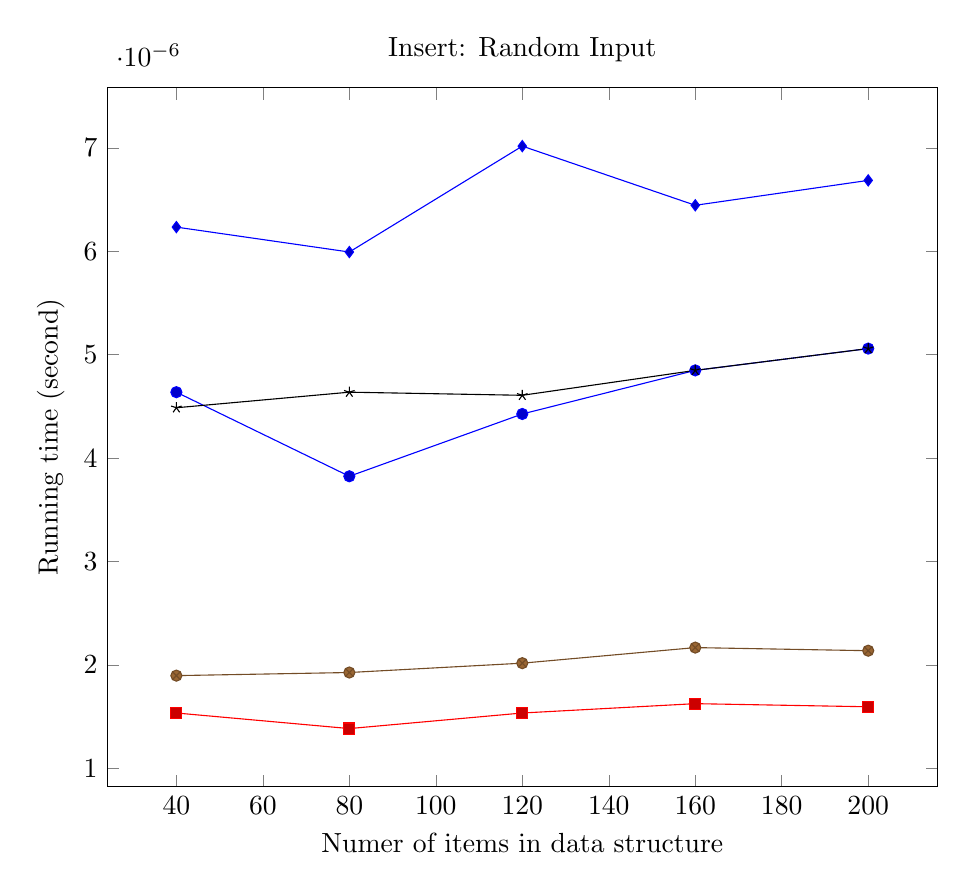
\begin{tikzpicture}
        \begin{axis}[
            xlabel={Numer of items in data structure},
            ylabel={Running time (second)},
            title={Insert: Random Input},
            width=\textwidth
        ]
		\addplot coordinates {
			(40, 4.638100185871963e-06)
			(80, 3.824926776729854e-06)
			(120, 4.427277450247402e-06)
			(160, 4.848922921851795e-06)
			(200, 5.059745657476355e-06)
		};
		\addplot coordinates {
			(40, 1.5359942175052766e-06)
			(80, 1.385406549303525e-06)
			(120, 1.5359942175052766e-06)
			(160, 1.6263468186394902e-06)
			(200, 1.5962292845728143e-06)
		};
		\addplot coordinates {
			(40, 1.89740462168686e-06)
			(80, 1.9275221553982645e-06)
			(120, 2.017874756177207e-06)
			(160, 2.1684624243789584e-06)
			(200, 2.1383448906675538e-06)
		};
		\addplot coordinates {
			(40, 4.487512517670212e-06)
			(80, 4.638100185871963e-06)
			(120, 4.6079826525158294e-06)
			(160, 4.848922921851795e-06)
			(200, 5.059745657476355e-06)
		};
		\addplot coordinates {
			(40, 6.234329470800048e-06)
			(80, 5.993389201464084e-06)
			(120, 7.017385346230754e-06)
			(160, 6.445152206424609e-06)
			(200, 6.686092476115846e-06)
		};
        \legend{}
        \end{axis}
    \end{tikzpicture}
    \caption{Average of 0 operations, benchmarked every 0, starting at 0.}
\end{figure}